%!TEX root = ../lectures_olympics.tex

\chapter{稳恒电流}

在过去已经学过很多和电路有关的物理过程,和电路的基本定律。
当把电压$U$加电阻$R$两端时,会有一定的电流$I$通过该电阻,它们之间由{\heiti 欧姆定律}{Ohm's Law}相联系:
\begin{equation}\label{eqn: 欧姆定律}
U=IR.
\end{equation}
利用欧姆定律可以解决很多电路相关的物理问题,现在我们将进一步深入地探讨电流的本质以及更复杂的电路。

\section{电流的微观解释}
{\heiti 电流}(currnent)并不仅存在于加了电源的闭合回路当中,实际上带电粒子无论何种形式的定向运动均会形成电流。
对于一个假想的截面$S$如果在$\Delta t$时间里通过该截面的电量为$\Delta Q$,通过该截面的电流$I$被定义为
\begin{equation}
I=\frac{\Delta Q}{\Delta t},
\end{equation}
更准确地,当通过该截面电量随时间的函数能够表达为$Q(t)$时,通过截面的电流为电量对时间的导数:
\begin{equation}\label{eqn: 电流的导数定义}
I(t)=\lim_{\Delta t\rightarrow 0}\frac{\Delta Q}{\Delta t}=\frac{dQ}{dt}(t),
\end{equation}
一般来说电流是时间的函数,如果电流不随时间而变的话,就称是一个{\heiti 稳恒电流}。
反过来当电流与时间关系为已知时,在$t_1$到$t_2$两个时刻之间通过截面的电量则可表达为电流对时间的积分:
\begin{equation}
Q(t_1\rightarrow t_2)=\int_{t_1}^{t_2}I(t)dt,
\end{equation}
对于电流为$I$的稳恒电流,在时间$t$里流过的电量$Q=It$。

在不同的条件下,物质导电的微观机制有很大的不同。
以下是几种常见的导电过程:
\begin{enumerate}
\item 最常见的电流现象自然是加了外电压的金属物质。
当加上外电压时在金属内部会产生电场,微观上看导体内有大量的自由电子,它们在电场作用下加速运动,又不断地与原子核发生碰撞而损失能量,最终达到宏观的稳定状态。
如果单位体积内能够自由运动的电子数为$n$,对于导体上一个面积为$S$的截面,如果通过它的电子定向运动的平均速度为$v$的话,根据电流的定义\ref{eqn: 电流的导数定义}可知通过截面的电流为
\begin{equation}
I=neSv,
\end{equation}
其中$e$为电子的电量。
电子与原子核的碰撞又把电子从电场当中得到的能量传递给导体,宏观上看在通电以后导体就会发热,也就是焦耳定律所陈述的事实。

\item 电解质溶液中以及熔融状态下的电解质中都有能参与导电的正、负离子,无外电场时它们的热运动并不表现为电流,当有外加电场作用下这些正负离子会做定向运动,宏观上看也形成了一个电流。
通过液体导电和微观解析能够迅速得到{\heiti 法拉弟电解定律}:
\begin{quotation}
电解质导电时,在极板上析出物质的质量与电流强度$I$和通电时间$t$的乘积成正比:
\begin{equation}
m=KIt = KQ
\end{equation}
式中$K$称为电化当量。
\end{quotation}


\item 在通常情况下,地表附近空气当中只包含的极少数的自由电荷,可以看做是绝缘体。
但是当空气当中电场或能量密度达到一定程度以后,在电场作用下气体分子会被“扯开”,也就是所谓的{\heiti 电离},此后在空气也变成了导体,在其内部会有电流,闪电就是一种典型的气体导电现象。
依靠外部条件,例如高温或紫外线照射而维持的气体导电过程称为气体的{\heiti 被激放电},反之如果气体分子是被外电场直接电离的导电过程则称为\emph{自激放电}。
地球大气层较高的部分由于持续受到太阳辐射和宇宙射线的碰撞,始终保持在电离状态,称做大气的{\heiti 电离层},电离层中的空气和地面不同,它们导体而不是绝缘体。


\item 形成电流其实并不一定需要介质,哪怕在真空中只要存在电荷的定向运动同样称之为一个电流。
宇宙射线就是真空中电流存在的一个典型例子,这些高能的带电粒子由天体过程产生,它们以接近光的速度通过真空射向宇宙当中各个区域。

\end{enumerate}


在中学阶段一般将电流当做标量来处理,但实际上根据电流的定义可以看出它实际上不仅依赖于带电粒子运动的速率,它们定向运动的方向同样是电流的一个重要属性。
准确地讲,当电流的方向与所研究问题无关时可以将其看做标量,但是当问题与电流的方向有关时必须认真地考虑其方向性,把它当做矢量来看待。

\begin{example}
如图所示的一个半径为$R$的刚性带电体沿着其对称轴以角速度$\omega$做匀速转动,该过程可以等效地看成一个电流$I$通过圆形导线,求该等效电流值。
\begin{flushright}
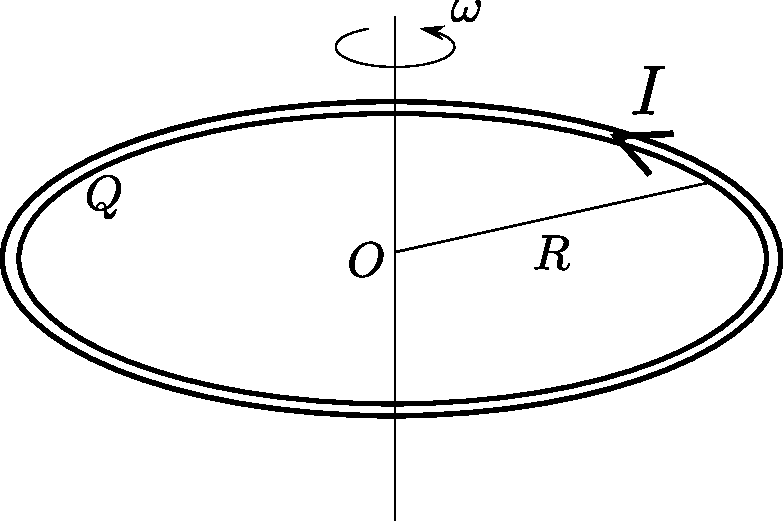
\includegraphics[width = 0.3\textwidth]{images/elec-current-1.pdf} 
\end{flushright}

\tagged{student}{\vspace*{0cm}}
\begin{taggedblock}{teacher}
\noindent
解析:带电体的线电荷密度$\lambda = Q/2\pi R$,在给定时间$\dt$里通过一个固定截面的电量
\[\Delta Q = \lambda \omega R \Delta t,\]
根据电流的定义可知等效电流
\[ I=\frac{\Delta Q}{\Delta t}=\lambda \omega R = \frac{Q\omega}{2\pi} \]
\end{taggedblock}
\end{example}

%%%%%%%%%%%%%%%
\begin{example}
	假设在导体中运动的电子受到一个正比于速度且与运动速度方向相反的阻力$f = -\alpha v$,证明在外电场作用下处于稳定状态的电流满足欧姆定律,并求出导体电阻率与阻力系数$\alpha$的关系。
	\tagged{student}{\vspace*{4cm}}
	\begin{taggedblock}{teacher}
		\newline
		解析:成正比
	\end{taggedblock}
\end{example}%%%
%%%%%%%%%%%%%%$$

\begin{example}
试根据导体导电的微观解释证明焦耳定律:当外电压为$U$,通过导体的电流为$I$时,导体在时间$t$内产生的热量$Q=UIt$
\tagged{student}{\vspace*{3cm}}
\begin{taggedblock}{teacher}
\newline
解析:最简单的假设下设导体为一个截面积为$S$、长度为$L$的圆柱体,当外接电压为$U$时它内部的电场强度$E=U/L$。
并且进一步假设当电流为$I$时所有的电子都以速度$v$做匀速直线运动:
\[ v=\frac{I}{neS}. \]
$\Delta t$时间里电场力对单个电子作功
\[\Delta W =  eEv\Delta t =\frac{U}{L}ev\Delta t\]
这样对所有载流电子所做的总功则是
\[ nSL\Delta W = neSv\cdot U\Delta t .\]
由于稳定的电子流动,这些功最终都由电子同原子核的碰撞转化成了导热的热能,所以单位时间里导体产生的热量,也就是热功率为
\[neSv\cdot U = UI. \]
\end{taggedblock}
\end{example}


\section{欧姆定律}
导体内部的电场会引起电子的定向运动,在外电压下电流与电压成正比,其关系由欧姆定律\ref{eqn: 欧姆定律}所给出。
电子在晶格之间运动,不断地与原子核发生碰撞\footnote{电子与原子的碰撞不是弹性碰撞,碰撞前后电子会损失能量},前后两次碰撞电子所行进的平均路程称为{\heiti 平均自由程}。
两次碰撞之间电子在外电场作用下做加速运动,金属当中所有电子都在作热运动和定向运动,其总的效果表现为一个宏观的电流。


实践上可以用电阻率来描写特定导体导电的性质,一般将电阻率记做$\rho$,对于一段长度为$L$,截面积为$S$的柱形导体来说,它的电阻可以由
\begin{equation}
R=\rho\frac{L}{S}
\end{equation}
所给出。
很明显可以看出,截面越大电阻越小、长度越大则电阻则越大。
电阻本质上是由金属中的原子与电子的碰撞所产生,它依赖于金属的微观结构。
电阻率代表着导电物质基本属性,它是由复杂的微观相互作用过程所决定。


\begin{example}
我们可以用一个简化的模型来描写导体中复杂的电子运动,将电子与某一导体中原子的碰撞简化地用一个正比于电子速度的阻力$f=-\alpha v$。
在这个简化模型当中,电子是在外部电场力和阻力作用下运动。
试证明阻力系数$\alpha$与该导体电阻率$\rho$之间的关系为$\alpha = ne^2\rho$,其中$n$为自由电子的数密度。


\tagged{student}{\vspace*{4cm}}
\begin{taggedblock}{teacher}
\noindent
解析:对于截面为$S$,长度为$L$的导体,它的电阻为$\rho\frac{L}{S}$,当外接电压为$U$时内部的电场强度为$E=U/L$,每个电子受电场力$f=eE$,它将与阻力平衡:
\[eE=\alpha v,\]
与此同时当平均速度$v$给定时电流为
\[I=neSv\]
其中$n$为电子的数密度。
将上面所有的量代入欧姆定律当中
\[EL = neSv\cdot \rho\frac{L}{S}=neS\frac{eE}{\alpha}  \rho\frac{L}{S}\]
将上式化简可得
\[
\alpha = ne^2\rho
\]
\end{taggedblock}
\end{example}




\section{简单电路}
在电路当中电阻有两种简单的连接方式,分别为电阻的串联和并联,其基本结构如图所示。
在稳恒电路当中通过多个串联电阻的电流均相同,设$n$个串联电阻的阻值分别为$R_1$、$R_2$,....,$R_n$,当电路当中当通过串联电路的电流为$I$,根据欧姆定律阻值为$R_i$两端的电压$U_i = IR_i$,串联电路两端的总电压则是每个电阻两端电压之和
\[
U=U_1+U_2+\dots +U_n = I(R_1+R_2+\dots +R_n)
\]
可以将它们等效地看做单独一个电阻,其阻值为
\begin{equation}
R=R_1+R_2+\dots +R_n。
\end{equation}


同理当多个电阻并联时,每个电阻两端的电压均相同,通过电阻$R_i$的电流可以根据欧姆定律
\begin{equation}
I_i = \frac{U}{R_i},
\end{equation}
这样通过并联电路的总电流
\[
I=I_1+I_2+\dots +I_n = \frac{U}{R_1}+\frac{U}{R_2}+\dots +\frac{U}{R_n},
\]
与欧姆定律相比较可以看出并联电阻的等效电阻
\begin{equation}
\frac{1}{R}=\frac{1}{R_1}+\frac{1}{R_2}+\dots+\frac{1}{R_n}
\end{equation}
所有能够分解成电阻串、并联的电路称为简单电路,可以利用串、并联的等效电阻求出通过所有电阻的电流。

\begin{example}
几个简单电路的例子
\tagged{student}{\vspace*{4cm}}
\begin{taggedblock}{teacher}
\newline
解析:略
\end{taggedblock}
\end{example}

\begin{example}
简单的无限电阻网格的等效电阻
\tagged{student}{\vspace*{4cm}}
\begin{taggedblock}{teacher}
\newline
解析:略
\end{taggedblock}
\end{example}

当电路当中包含有电源时,和过去我们所处理的电源稍有不同的是,现实的电源除了提供电动势以外还可能会由其内部结构带有一定的电阻,称做电源的{\heiti 内阻}。
这样对于图所示的一段电路,设电源的电动势为$\mathcal{E}$,内阻为$r$,外接一个阻值为$R$的电阻时电路当中的电流为
\begin{equation}
I=\frac{\mathcal{E}}{R+r},
\end{equation}
其它复杂电路中电流的求解也遵循类似的方法。




\section{复杂电路,基尔霍夫定律}

\section{电压表、电流表和欧姆表}
为了能够探测电路中的电流和电压或给定电阻的阻值,我们需要在通电的电路中接入用来测量这些电学量的仪器,这们设计的基本思想都是对微弱电流的测量而确定电路的性质。
用来测量微弱电流的电表称为{\heiti 灵敏电流计},它能够在很高精度内测量很小的电流,但是允许通过它的最大电流,也就是额定电流通常很小,并且具有一定的电阻$R_g$,称为灵敏电流表的内阻。
为了在更大的范围内测量电路的性质,或测量其它物理量,需要对灵敏电流表做一定的改装,根据测量目的的不同典型的改装后的电表包括{\heiti 电流表}、\emph{电压表}以及\emph{欧姆表}等。
一个需要特别注意的是当把电表接入电路以后,它必然会改变原有电路的电流分布,所以它们的读数与真实值之间有一定的偏差,这是利用各种电表进行电路测量中的{\heiti 系统误差}的主要来源。
常见的电表包括
\begin{enumerate}
\item 电流表:其电路如图,将一个灵敏电流计和一个定值电阻$R_S$并联,$R_S$的目的是为了分流以避免灵敏电流计过载。
这时通过灵敏电流计的电流和原始电路当中电流$I$之间满足关系
\begin{equation}
I_g = \frac{R_S}{R_S+R_g}I,
\end{equation}
从中可以看出通过减小$R_S$来增加电流表的量程,并且减小电流表的等效电阻从而降低对接入电路的影响。


\item 电压表:将一个电阻$R_m$与灵敏电流表串联就形成最简单的电压表,其电路如图所示。
串联电阻用来分压以避免灵敏电流计过载并且提高电压表的电阻使其对电路的影响降到最小。

\end{enumerate}

\begin{example}
伏安法测电阻的误差分析
\tagged{student}{\vspace*{4cm}}
\begin{taggedblock}{teacher}
\newline
解析:略
\end{taggedblock}
\end{example}

\begin{example}
改装电表的例子
\tagged{student}{\vspace*{4cm}}
\begin{taggedblock}{teacher}
\newline
解析:略
\end{taggedblock}
\end{example}

\section{惠斯通电桥和补偿电路}

\section{半导体简介}
